\documentclass{beamer}

\usepackage{ucs}
\usepackage[utf8x]{inputenc}
\usepackage[T1]{fontenc}
\usepackage[english]{babel}

\usepackage[retainorgcmds]{IEEEtrantools}%	IEEEeqnarray

\usepackage{mathabx}%	convolution symbol
\usepackage{multi row}
\usepackage{epstopdf}
\usepackage{listings}
\lstset{
	language=c,
	basicstyle=\footnotesize,
	showtabs=true,
	tabsize=3,
}

%	presentation info
\title{Projecto Integrado - Apresentação Intermédia 3}

\author{António Silva, Rui Brito}

\institute[pg22820, pg22781]{
	Universidade do Minho
}

\date{Braga, Maio 2013}


%	beamer options
\usetheme{Frankfurt}


\begin{document}%	begin presentation

\maketitle%	title slide

\begin{frame}
	\frametitle{Índice}
	\tableofcontents
\end{frame}

\section{Modificações}
\begin{frame}
	\frametitle{Modificações na BD}

	\begin{figure}[!htp]
		\includegraphics[totalheight=1.2\textheight,angle=90]{../bd3.eps}		
		\end{figure}

\end{frame}

\begin{frame}
	\frametitle{Parser BibTeX}
	\begin{itemize}
		\item Módulo reescrito desde a fase anterior;
		\item Todos os dados são inseridos na BD;
		\item Entradas organizadas por key e não por autor;
		\item Tratamento de actualizações;		
	\end{itemize}
		
	
\end{frame}

\begin{frame}
	\frametitle{Interface Única}
	\begin{itemize}
		\item Implementação em PHP, usando AngularJS e Twitter Bootstrap;
		\item Remodelação da interface de publicações
		\item Carregamento dos dados directamente da BD
	\end{itemize}
\end{frame}
\begin{frame}
	\frametitle{Interface Única}
	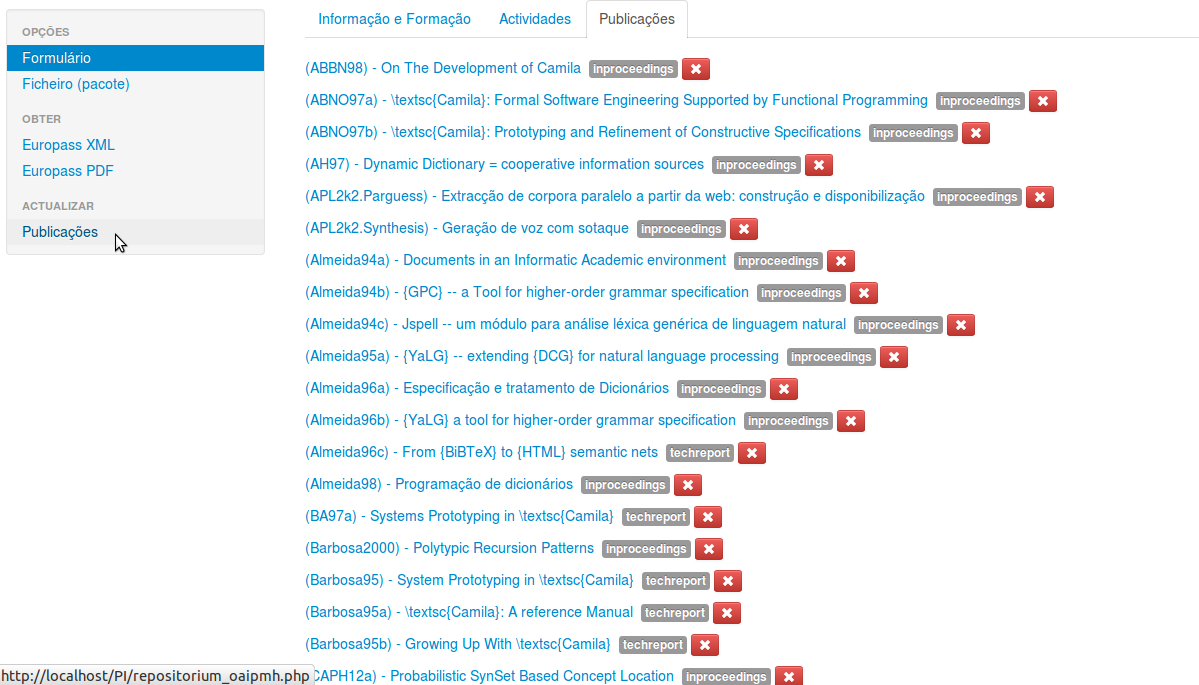
\includegraphics[width=1.2\textwidth]{../iPublications2.png}
\end{frame}

\section{Europass}
\begin{frame}
	\frametitle{Europass XML}
	\begin{itemize}
		\item Versão 2 vs Versão 3
		\item Exportação de publicações e actividades
		\item Exportação da fotografia
	\end{itemize}
\end{frame}
\begin{frame}
	\frametitle{Europass PDF}
	\begin{itemize}
		\item Web Service (ou falta dele)
		\item Uso do editor oficial
		\item Tentativa de geração de JSON
	\end{itemize}
\end{frame}

\section{RepositoriUM}
\begin{frame}
	\frametitle{Importação de publicações}
	\begin{itemize}
		\item Tempo de acesso
		\item Actualização e inserção baseada em intervalos temporais
		\item Possiblidade de reset por parte do utilizador
		\item Utilização de uma pequena classe intermediária
		
	\end{itemize}
\end{frame}

\section{Web Semântica}
\begin{frame}
	\frametitle{RDFa}
	\begin{itemize}
		\item Utilização de propriedades da classe Person definidas no schema.org
		\begin{itemize}
			\item name
			\item birthDate
			\item gender
			\item email
			\item telephone
		\end{itemize}
		\item Não foram desenvolvidas novas ontologias paras as actividades nem para as Publicações
	\end{itemize}
\end{frame}


\begin{frame}
	\begin{center}
		\Huge\bfseries
		Demo
	\end{center}
\end{frame}

\section{Questões}
\begin{frame}
\titlepage
	\begin{center}
		\Huge\bfseries
		- ? -
	\end{center}
\end{frame}

\end{document}%	end presentation
